% B4.1 -- Part 1: interpretation of the two experiments (concise)
\setsecblurb{Two regimes, same backbone, same questions.\\the prediction failed; what replaced it is a better claim.}
\section{What the two experiments say}

\begin{frame}[t]{Design summary}{Same backbone, same questions, different memory architecture}
  \footnotesize
  \begin{tabular}{@{}p{1.1cm}p{4.4cm}p{2.0cm}@{}}
    \toprule
    & \thead{how context reaches the model} & \thead{scored records} \\
    \midrule
    \Eone & re-encodes the whole window at every checkpoint & \NrecEone \\
    \Etwo & one ingestion into a bounded KV cache, queried at checkpoints & \NrecEtwo \\
    \bottomrule
  \end{tabular}
  \vskip0.6em
  {\footnotesize Same frozen Qwen3-VL-8B, same \Nquestions\ EgoLifeQA questions, same frame bank, same analysis code. EgoStream is a plug-in memory manager over the same weights --- no bridge condition needed.}
  \vskip0.4em
  \claim{\footnotesize \acc{Accuracy}: argmax vs gold. \conf{Confidence}: max softmax$(\{$A,B,C,D$\})$ at the first generated position; no text generated. Every $\Delta$ is a \textbf{paired within-question contrast}, cluster-bootstrapped over questions (5{,}000 draws).}
\end{frame}

\begin{frame}[t]{The predicted signature is absent in both regimes}{The recommendation is to retire the original hypothesis}
  \claim{\textbf{Prediction:} the gap between confidence and accuracy \emph{widens} as evidence ages.}
  \vskip0.8em
  \begin{center}\footnotesize
    \begin{tabular}{@{}lcc@{}}
      \toprule
      \thead{overconfidence gap, \dt\ 1\,$\rightarrow$\,60 min} & \thead{change (pp)} & \thead{$p$} \\
      \midrule
      \Eone\ --- full-reprocess & \EoneGap & \EoneGapP \\
      \Etwo\ --- streaming KV cache & \EtwoGap & \EtwoGapP \\
      \bottomrule
    \end{tabular}
  \end{center}
  \vskip0.8em
  {\footnotesize Both point mildly toward \emph{narrowing}. \Etwo\ was the setting the hypothesis most deserved --- a bounded cache actually destroys the evidence --- and it still did not appear.}
\end{frame}

\begin{frame}[t]{\Eonelong: confidence tracks the wrong variable}
  \begin{columns}[T]
    \begin{column}{0.42\textwidth}
      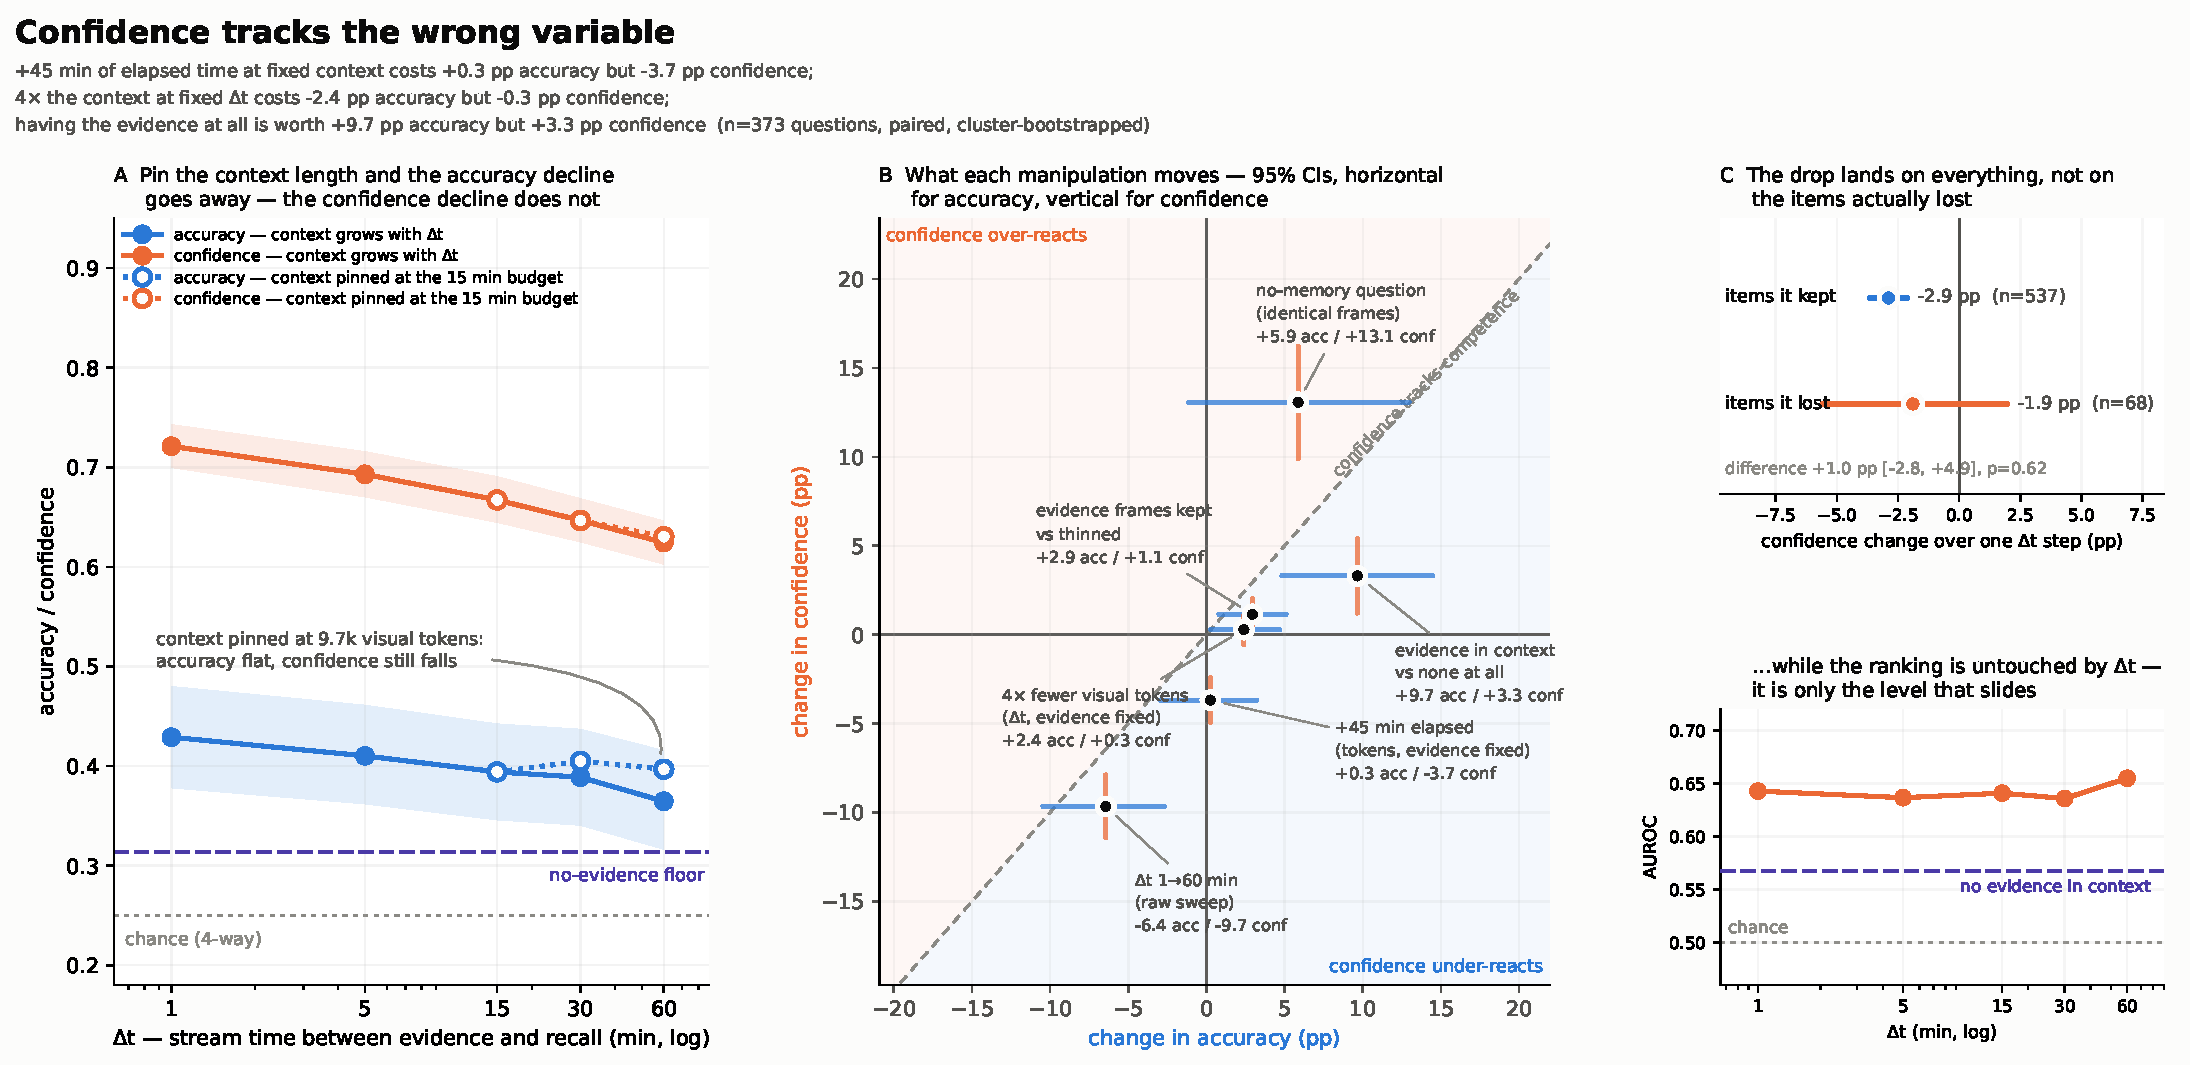
\includegraphics[width=\linewidth,height=0.68\textheight,keepaspectratio]{figures/e1-full.pdf}
    \end{column}
    \begin{column}{0.56\textwidth}
      \footnotesize
      \begin{tabular}{@{}p{2.6cm}rr@{}}
        \toprule
        \thead{manipulation} & \thead{\acc{$\Delta$acc}} & \thead{\conf{$\Delta$conf}} \\
        \midrule
        $+$45 min elapsed \newline\emph{\scriptsize(tokens fixed)} & \EoneElapsedAcc & \EoneElapsedConf \\[0.3em]
        4$\times$ fewer tokens \newline\emph{\scriptsize(\dt\ fixed)} & \EoneTokensAcc & \EoneTokensConf \\[0.3em]
        evidence vs none \newline\emph{\scriptsize(token-matched)} & \EoneEvidenceAcc & \EoneEvidenceConf \\
        \bottomrule
      \end{tabular}
      \vskip0.5em
      \claim{\scriptsize \conf{Confidence} moves on elapsed time, which costs \emph{no} accuracy. \acc{Accuracy} moves on context length and evidence, which confidence barely registers.}
    \end{column}
  \end{columns}
  \source{\texttt{figures/headline.pdf} (M7). Nothing redrawn.}
\end{frame}

\begin{frame}[t]{\Etwolong: the same dissociation, rotated}{Accuracy responds to evidence; confidence responds to context volume}
  \begin{columns}[T]
    \begin{column}{0.48\textwidth}
      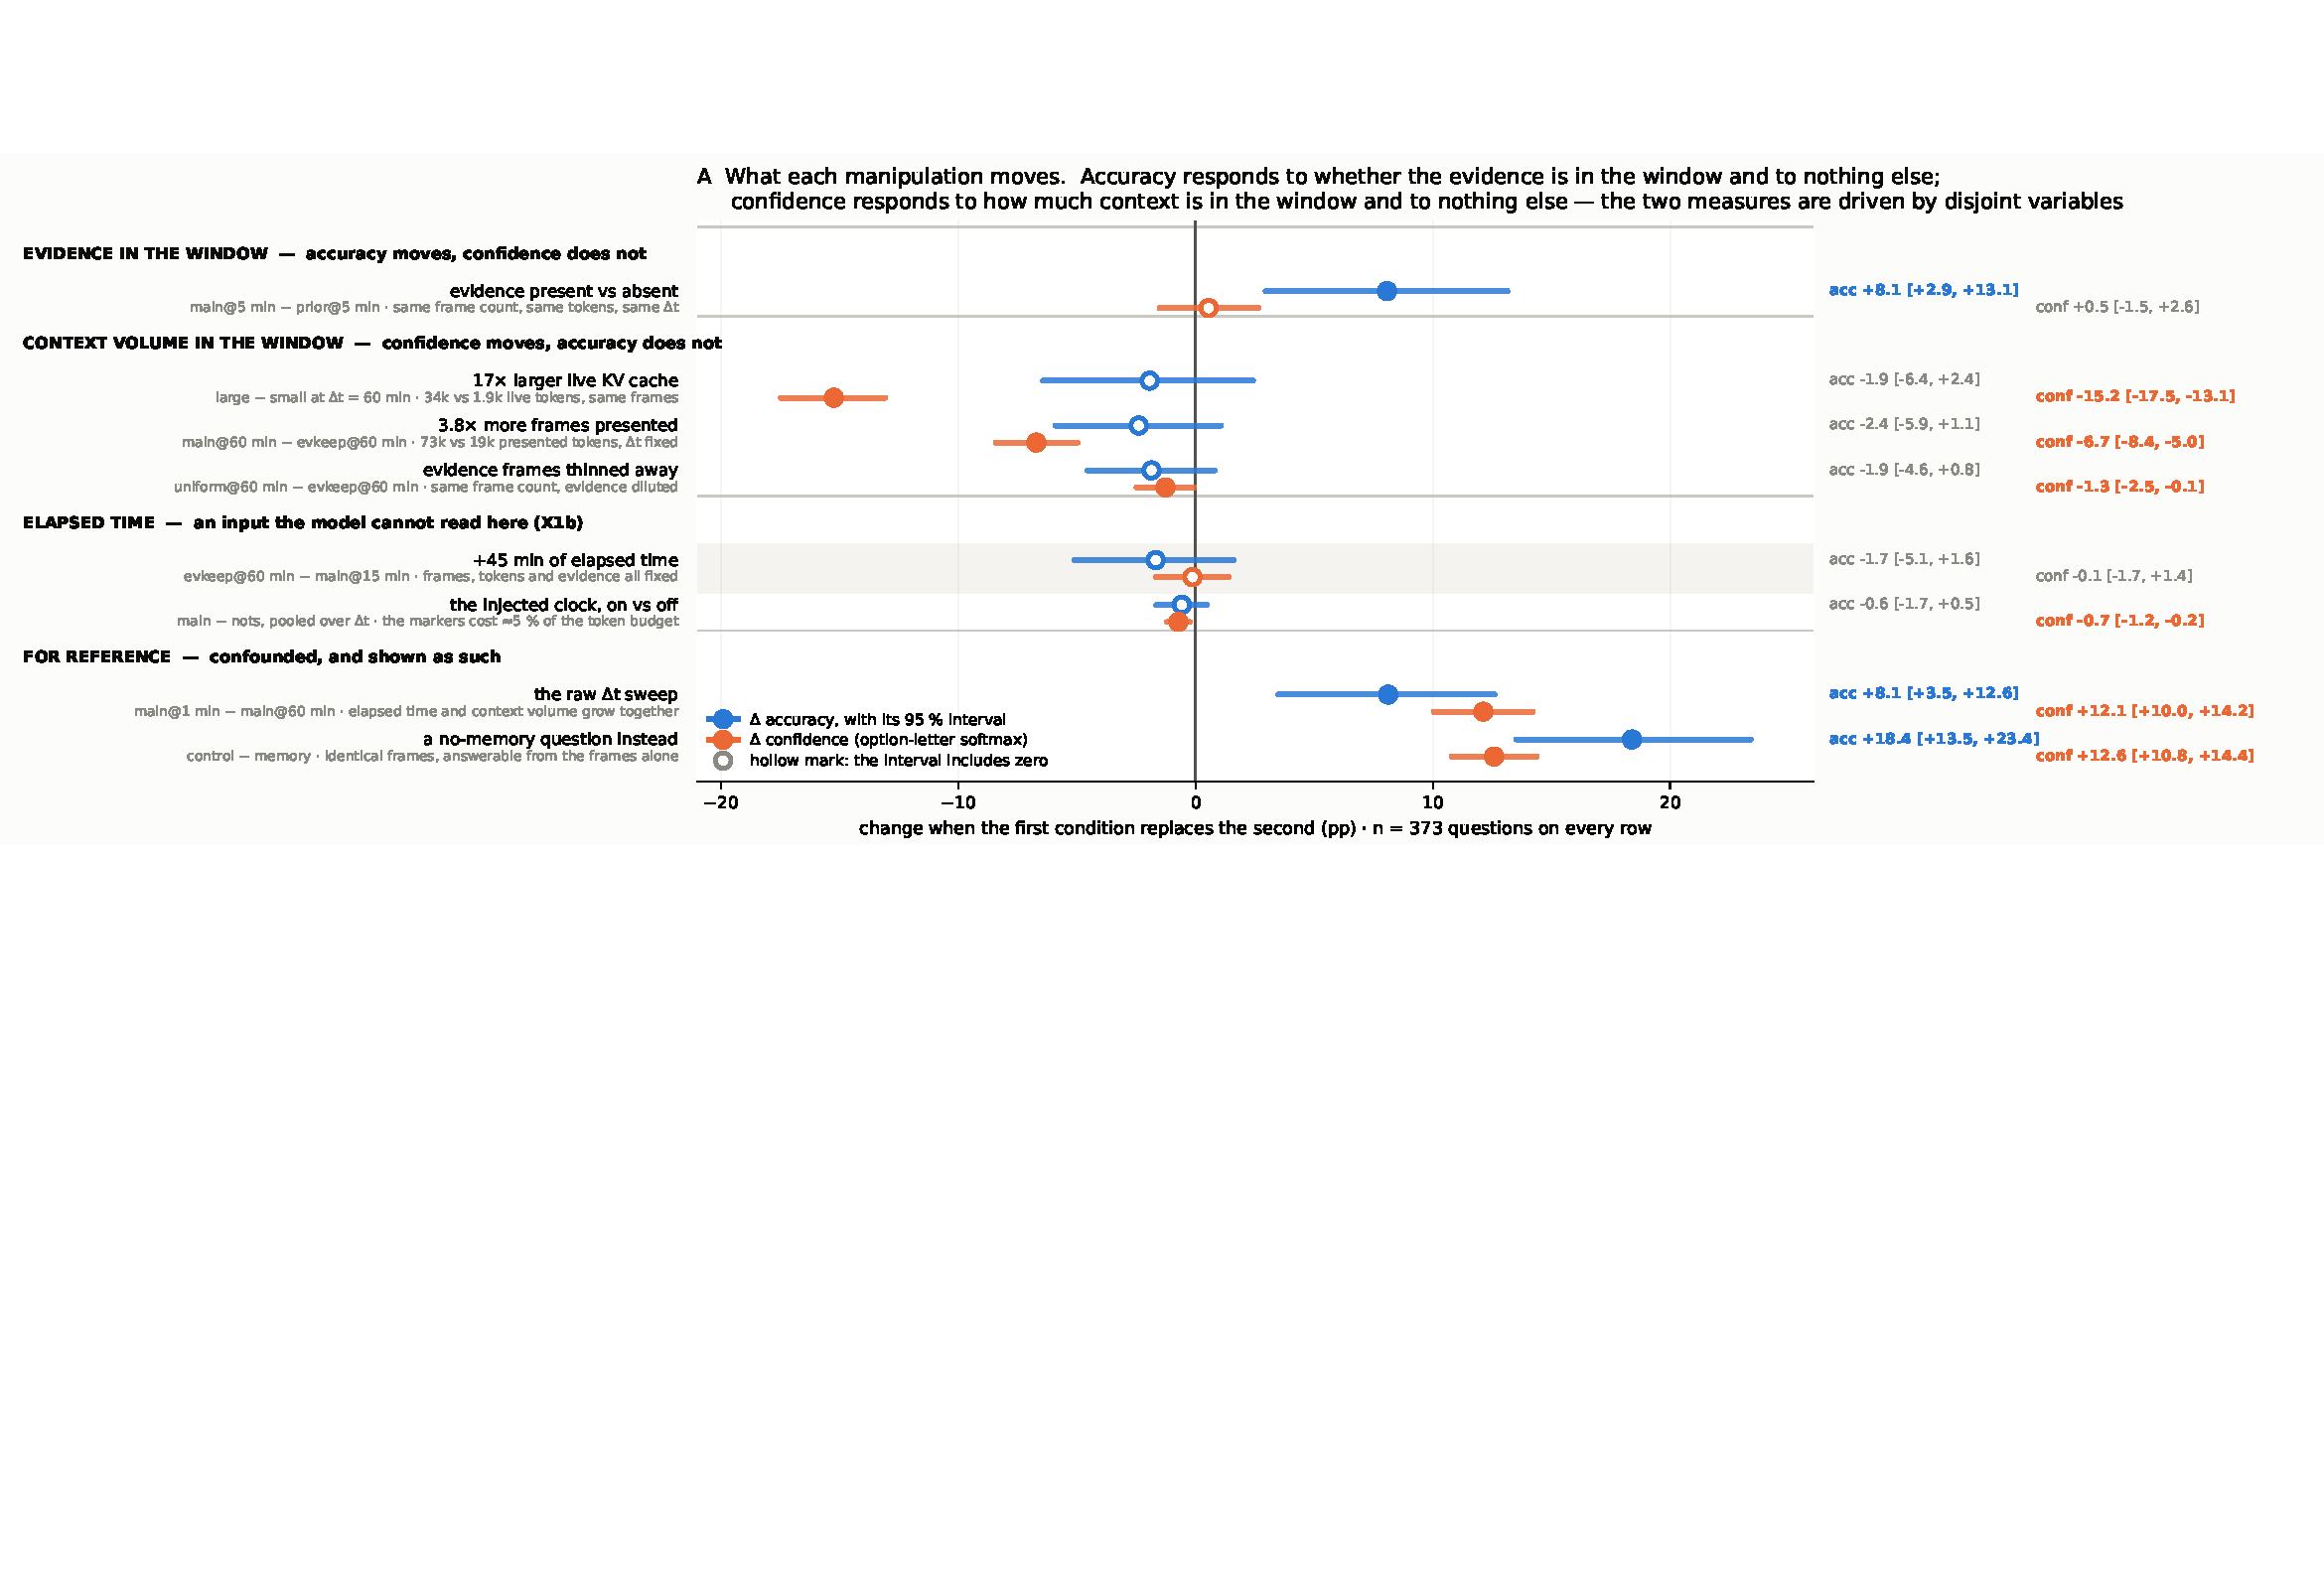
\includegraphics[width=\textwidth,height=0.62\textheight,keepaspectratio]{figures/e2-a.pdf}
      \vskip0.3em
      {\scriptsize\color{inkmid}Elapsed-time axis is \emph{unavailable}, not null --- see backup.}
    \end{column}
    \begin{column}{0.50\textwidth}
      {\footnotesize\textbf{Budget dose--response at \dt\ = 60 min:}}
      \vskip0.3em
      \scriptsize
      \begin{tabular}{@{}crr@{}}
        \toprule
        \thead{\dt\ (min)} & \thead{\acc{$\Delta$acc}} & \thead{\conf{$\Delta$conf}} \\
        \midrule
        \TabEtwoBudgetNarrow
        \bottomrule
      \end{tabular}
      \vskip0.5em
      \claim{\scriptsize A \EtwoBudgetRatio\ live-token budget is worth \acc{\EtwoBudgetAcc} of accuracy and \conf{\EtwoBudgetConf} of confidence. Monotone on one measure, flat on the other.}
    \end{column}
  \end{columns}
  \source{\texttt{figures/streaming\_headline.pdf} (X10). Full figure in backup.}
\end{frame}

\begin{frame}[t]{Cross-regime: the dissociation replicates and its driver rotates}{Differenced contrasts --- same manipulation in both regimes, paired on the same questions}
  \begin{center}\footnotesize
    \begin{tabular}{@{}p{5.2cm}rrr@{}}
      \toprule
      \thead{manipulation, $\Delta$confidence} & \thead{\Eone} & \thead{\Etwo} & \thead{difference (\Etwo\,$-$\,\Eone)} \\
      \midrule
      \TabCrossRegime
      \bottomrule
    \end{tabular}
  \end{center}
  \vskip0.5em
  \begin{columns}[T]
    \begin{column}{0.49\textwidth}
      {\footnotesize\textbf{Invariant.} Accuracy responds to evidence presence; confidence does not --- in either regime.}
    \end{column}
    \begin{column}{0.49\textwidth}
      {\footnotesize\textbf{Rotated.} In \Eone\ confidence slid with elapsed time; in \Etwo\ it slides with context volume. Both differences exclude zero.}
    \end{column}
  \end{columns}
\end{frame}

\begin{frame}[t]{Unified account and implications}
  \claim{\footnotesize\textbf{Confidence is computed from surface properties of the context} --- how much visual input was processed (retained or not), and how long ago it says that was --- \textbf{not from whether the needed information is present.} Remove one surface cue and it latches onto another. What it never latches onto is evidence.}
  \vskip0.6em
  {\footnotesize\textbf{What this does to the original claim:}}
  \begin{itemize}\footnotesize\setlength\itemsep{0.15em}
    \item \textbf{Half 1} (``widening gap as evidence ages'') --- {\color{flagred}rejected twice.}
    \item \textbf{Half 2} (``\dt-conditioned recalibration recovers reliability'') --- {\color{flagred}needs revision.} \dt\ is the wrong conditioner; it worked in \Eone\ by accident. The variable that actually drives confidence is \texttt{live\_tokens}.
    \item \textbf{Headroom differs by regime.} AUROC is flat over the \Eone\ sweep (\EoneAurocDelta) but decays in \Etwo\ (\EtwoAurocDelta, $p$ = \EtwoAurocP). Recalibrating a level only works if the ranking survives.
  \end{itemize}
  \vskip0.3em
  {\footnotesize\color{goodgreen}The cheap fix looks cheaper the less realistic the memory system is --- only visible because both regimes were run.}
\end{frame}
